% Define document class
\documentclass[modern]{aastex631}

% Custom defs
% Packages
\usepackage{xifthen}
\usepackage{array}
\usepackage{upgreek}
\usepackage[bbgreekl]{mathbbol}
\usepackage{afterpage}
\usepackage[bb=boondox]{mathalpha}
\usepackage{tipa}
\usepackage{booktabs}


% Shorthand for this paper
\newcommand{\starry}{\textsf{starry}\xspace}
\newcommand{\Python}{\textsf{Python}\xspace}
\newcommand{\cpp}{\textsf{C}++\xspace}
\newcommand{\bvec}[1]{{\ensuremath{\mathbf{#1}}}}
\newcommand{\xxx}[1]{{\color{red}#1}}
\DeclarePairedDelimiter\floor{\lfloor}{\rfloor}
\DeclarePairedDelimiter\ceil{\lceil}{\rceil}
\newcommand{\imag}{{\ensuremath{\mathbb{i}}}}
\renewcommand{\quad}{\hskip 0.33em}
\newcommand{\quadquad}{\quad\quad\quad\quad}

\newcommand{\R}{\bvec{R}}
\newcommand{\AOne}{\bvec{A_1}}
\newcommand{\alm}{\bvec{a}}
\newcommand{\x}{\bvec{x}}
\newcommand{\D}{D}
\newcommand{\Doppler}{\bvec{D}}
\newcommand{\Surf}{\mathcal{S}}
\newcommand{\Curve}{\mathcal{C}}
\newcommand{\Dargs}{\bvec{d}}
\newcommand{\lmax}{\ensuremath{l_\mathrm{max}}}
\newcommand{\spot}{\texttt{SPOT}\xspace}
\newcommand{\vogtstar}{\texttt{VOGTSTAR}\xspace}
\newcommand{\kT}{\boldsymbol{\kappa}^\top}
\newcommand{\rhoT}{\boldsymbol{\rho}^\top}
\newcommand{\ylmbasis}{\boldsymbol{\psi}^\top}
\newcommand{\pbasis}{\boldsymbol{\phi}^\top}
\newcommand{\pbasisn}{\ensuremath{\phi_n}}
\newcommand{\almt}{\ensuremath{\bvec{a}}}
\newcommand{\lnlam}{\mbox{\textipa{\textcrlambda}}}

% Begin!
\begin{document}

% Title
\title{A Closed-Form Solution to the Doppler Imaging Problem}

% Author list
\author[0000-0002-0296-3826]{Rodrigo Luger}
\email{rluger@flatironinstitute.org}
\affil{Center~for~Computational~Astrophysics, Flatiron~Institute, New~York, NY}
%
\author{Megan Bedell}
\affil{Center~for~Computational~Astrophysics, Flatiron~Institute, New~York, NY}
%
\author{Daniel Foreman-Mackey}
\affil{Center~for~Computational~Astrophysics, Flatiron~Institute, New~York, NY}
%
\author{David W. 
Hogg}
\affil{Center~for~Computational~Astrophysics, Flatiron~Institute, New~York, NY}

\begin{abstract}
    We derive a closed form, analytic solution to the problem of Doppler imaging of stellar surfaces in the limit of negligible differential rotation and convective blueshift.
    The model for the observed spectrum is linear in the coefficients of the spherical harmonic expansion of the specific intensity distribution on the surface and, in certain limits, the posterior over surface maps has a closed form, analytic solution that is computationally trivial to evaluate.
    The model is also linear in the local (rest frame) stellar spectrum, which may itself be spatially variable.
    This allows one to perform Doppler imaging without knowledge of the local stellar spectrum and therefore works on blended lines or regions of the spectrum where line formation mechanisms are not well understood.
    Finally, the model is fast, differentiable, and allows one to calculate uncertainties on the inferred surface map.
\end{abstract}

% Main body
\section{Introduction}
The paper is organized as follows: in \S\ref{sec:the_problem}~and~\S\ref{sec:the_solution} we introduce the math behind the Doppler imaging problem and derive a closed form expression for the model. 
In \S\ref{sec:linear},~\S\ref{sec:inverse},~and~\S\ref{sec:bellswhistles} we demonstrate how to re-express the model as a linear operation on the input spectrum and stellar map and derive closed form expressions for the two conditioned on the data and priors.
In \S\ref{sec:spotstar} we apply our techniques to a mock problem. 
We further discuss and summarize our results in \S\ref{sec:discussion}~and~\S\ref{sec:conclusions}. 
Finally, auxiliary derivations are presented in the Appendix.

\section{The problem}
\label{sec:the_problem}
%
Let $I(\lnlam, \x, t)$ be the specific intensity observed at log wavelength $\lnlam \equiv \ln\frac{\lambda}{\lambda_\mathrm{r}}$ and at sky-projected Cartesian position $\x = (x, y, z)$ on the surface of the star at time $t$, where $\lambda_\mathrm{r}$ is a reference wavelength.
We may express this intensity as
%
\begin{align}
    \label{eq:the_problem:Ixi}
    I(\lnlam, \x, t) & =
    I\Big(\lnlam_0 + \D(\x), \x, t\Big)
\end{align}
%
where $\lnlam_0$ is the log wavelength in the rest frame and $\D$ is the Doppler shift in log wavelength space:
%
\begin{align}
    \label{eq:the_problem:D}
    \D(\x)
     & =
    \frac{1}{2}\ln\left(
    \frac{1 + \beta(\x)}{1 - \beta(\x)}
    \right)
\end{align}
%
where $\beta = v(\x) / c$ is the ratio of the radial velocity at a point on the surface of the star to the speed of light.
In keeping with the literature, we take positive values of $v$ (and $\D$) to mean redshifts.

A common approach to computing the Doppler-shifted spectrum is to evaluate the spectrum at the rest frame wavelength $\lnlam_0$ and interpolate back to the grid in $\lnlam$. 
This is practical when computing the spectrum at a single \emph{point} on the surface, but not ideal when one is interested in the \emph{integral} over the visible surface of the star $\Surf$, which is typically all we can observe:
%
\begin{align}
    \label{eq:the_problem:F}
    F(\lnlam, t)
     & \equiv
    \iint\limits_{\Surf(\x)}
    I(\lnlam, \x, t)
    \mathrm{d}{\Surf(\x)}
    \quad,
\end{align}
%
The difficulty in solving Equation~(\ref{eq:the_problem:F}) stems from the fact that $I(\lnlam, \x, t)$ is difficult to write down in closed form, given the nonlinearity of the Doppler shift.
The standard approach to solving this integral is therefore to discretize the surface of the star with a fine grid, evaluate the Doppler-shifted spectrum in each cell, and sum over the spatial axes to approximate the integral. 
Depending on the resolution of the grid, this is either numerically inaccurate or computationally inefficient (and often both).

\section{The Solution}
\label{sec:the_solution}

\subsection{Doppler Deconvolution}

The observed spectrum is a complex function of spatial, spectral, temporal, and velocity terms. 
The goal in this section is to deconvolve each of these terms to make solving the integral in Equation~(\ref{eq:the_problem:F}) easier.
%
The first thing we will do is to express Equation~(\ref{eq:the_problem:Ixi})
as a convolution:
%
\begin{align}
    \label{eq:deconv:convolution}
    I(\lnlam, \x, t) & =
    I(\lnlam_0, \x, t)
    *
    \delta\big(\lnlam_0 + \D(\x)\big)
\end{align}
%
where $\delta$ is the Dirac delta function and $*$ denotes the linear convolution operator, defined for two arbitrary functions $g$ and $h$ as the integral
%
\begin{align}
    \label{eq:deconv:convolution_def}
    (g * h)(t) \equiv \int_{-\infty}^\infty g(\tau) h(t - \tau) d\tau
\end{align}
%
for some independent coordinate $t$ and dummy parameter $\tau$.
%
The convolution of $I(\lnlam_0)$ with a delta function has the effect of shifting the spectrum by an amount $\D$, returning a function of the shifted (observed) log wavelength, $\lnlam = \lnlam_0 + \D$.

Next, we expand the spatial dependence of the specific intensity at the rest frame wavelength in terms of spherical harmonics on the unit disk:
%
\begin{align}
    \label{eq:deconv:Ixi0}
    I(\lnlam_0, \x, t)
     & =
    \sum_{l=0}^{l_\mathrm{max}}\sum_{m=-l}^{l} a_{lm}(\lnlam_0, t) Y_{lm}(\x)
    \quad ,
\end{align}
%
where $Y_{lm}(\x)$ is a spherical harmonic on the projected disk and $a_{lm}(\lnlam_0, t)$ is the corresponding spherical harmonic coefficient at log wavelength in the rest frame $\lnlam_0$ and time $t$. 
For convenience, we may write this equation in vector form:
%
\begin{align}
    \label{eq:deconv:Ivec}
    I(\lnlam_0, \x, t) & =
    \ylmbasis(\x) \,
    \almt(\lnlam_0, t)
    \quad ,
\end{align}
%
where
%
\begin{align}
    \label{eq:deconv:almt}
    \almt(\lnlam_0, t) \equiv
    \Big(
    a_{0,0}(\lnlam_0, t) \quad 
    a_{1,-1}(\lnlam_0, t) \quad 
    a_{1,0}(\lnlam_0, t) \quad 
    a_{1,1}(\lnlam_0, t) \quad
    ...
    \Big)^\top
\end{align}
%
is the vector of $N = (l_\mathrm{max} + 1)^2$ spherical harmonic coefficients and
%
\begin{align}
    \label{eq:deconv:ylmbasis}
    \ylmbasis(\x) \equiv
    \Big(
    Y_{0,0}(\x) \quad 
    Y_{1,-1}(\x) \quad 
    Y_{1,0}(\x) \quad 
    Y_{1,1}(\x) \quad
    ...
    \Big)
\end{align}
%
is the corresponding vector of $N$ spherical harmonics. 
We may further decompose our expression by linearizing the time dependence of the spherical harmonic coefficients:
%
\begin{align}
    \label{eq:deconv:R}
    \almt(\lnlam_0, t) = \R(t) \, \alm(\lnlam_0)
    \quad ,
\end{align}
%
where $\alm(\lnlam_0) = \bvec{a}(\lnlam_0, t=t_0)$ for some reference time $t_0$.
For rigid body rotation, the result is exact and $\R(t)$ is the $(N \times N)$ Wigner rotation matrix for real spherical harmonics
\citep[e.g.][]{AlvarezCollado1989}, which is implicitly a function of the inclination, obliquity, and rotation period of the star.
%In the case that other processes such as differential rotation or spot 
%evolution are significant
%over the course of an observation, Equation~(\ref{eq:deconv:R}) can be
%made to hold approximately for some effective rotation matrix 
%$\R(t)$; we discuss this later.

The equation for the specific intensity in the rest frame now reads
%
\begin{align}
    \label{eq:deconv:Ivecfull}
    I(\lnlam_0, \x, t) & =
    \ylmbasis(\x)
    \,
    \R(t)
    \,
    \alm(\lnlam_0)
    \quad ,
\end{align}
%
where it is clear that we have fully separated the spatial, temporal, and spectral terms. 
Inserting this into Equation~(\ref{eq:deconv:convolution})
and integrating over the visible portion of the star, we arrive at the expression for the observed spectrum:
%
%
\begin{align}
    \label{eq:deconv:F2d}
    F(\lnlam, t) & =
    \iint\limits_{\Surf(\x)}
    \ylmbasis(\x)
    \,
    \R(t)
    \,
    \almt(\lnlam_0)
    * \delta\big(\lnlam_0 + \D(\x)\big)
    \mathrm{d}\Surf(\x)
    \nonumber                \\[0.5em]
                         & =
    \iint\limits_{\Surf(\x)}
    \ylmbasis(\x)
    \delta\big(\lnlam_0 + \D(\x)\big)
    \mathrm{d}\Surf(\x)
    \,
    \R(t)
    \,
    *
    \,
    \alm(\lnlam_0)
    \quad ,
\end{align}
%
%
where we made use of the commutativity of the convolution operator and the fact that the integral is taken only over the spatial dimensions.
Note, importantly, that the convolution operation above is implicitly a vector operation---i.e., the convolution is taken for each spherical harmonic term individually and then summed over all terms.

Finally, we can simplify Equation~(\ref{eq:deconv:F2d}) by noting that the delta function in the integrand allows us to reduce the double integral to a line integral:
%
\begin{align}
    \label{eq:deconv:kT}
    \iint\limits_{\Surf(\x)}
    \ylmbasis(\x)
    \delta\big(\lnlam_0 + \D(\x)\big)
    \mathrm{d}\Surf(\x)
    \, \,
     & =
    \int\limits_{\Curve(\lnlam, \x)}
    \hspace*{-0.6em}\ylmbasis(\x)
    \mathrm{d}\Curve(\lnlam, \x)
    \nonumber                     \\[0.5em]
     & \equiv \kT(\lnlam)
    \quad.
\end{align}
%
where the path $\Curve(\lnlam, \x)$ corresponds to the set of all points on the visible disk where $\lnlam_0 + \D(\x) = 0$.
%
We thus have
%
\begin{align}
    \label{eq:deconv:F}
    F(\lnlam, t)
     & =
    \kT(\lnlam) \, \R(t)
    *
    \alm(\lnlam_0)
    \quad.
\end{align}
%
Equation~(\ref{eq:deconv:F}) is the deconvolution of the observed spectrum into velocity terms, temporal terms, and spectral/spatial terms, respectively. 
In the next section, we will discuss how to efficiently solve the line integral in Equation~(\ref{eq:deconv:kT}).

\subsection{Computing the kernel $\kT$}
\label{sec:kT}
%
In the case that the star's rotation is rigid (i.e., differential rotation is negligible) and other effects such as convective blueshift may be ignored, the radial velocity at any point on the surface is simply proportional to the distance to the axis of rotation. 
Without loss of generality, if we assume the axis of rotation lies along the $y-z$ plane, we have
%
\begin{align}
    \label{eq:kT:beta}
    \beta(\x) = \frac{\omega \sin i \, x}{c}
\end{align}
%
and
%
\begin{align}
    \label{eq:kT:D}
    \D(\x) & =
    \frac{1}{2}\ln\left(
    \dfrac{1 + \dfrac{\omega \sin i \, x}{c}}
    {1 - \dfrac{\omega \sin i \, x}{c}}
    \right)
    \quad ,
\end{align}
%
where $\omega$ is the stellar angular velocity and $i$ is the stellar inclination with respect to $\hat{y}$.

\begin{figure}[t!]
    \begin{centering}
        \includegraphics[width=\linewidth]{figures/kT.pdf}
        \caption{%
            The Doppler $\kT$ basis for a rigidly rotating star computed from Equation~(\ref{eq:kT:kT}) and Equation~(\ref{eq:kT:sTrecurrence}) up to spherical harmonic degree $l_\mathrm{max}=10$. 
            Rows correspond to the degree $l$ and columns correspond to the order $m$. 
            These functions encode the contribution of each spherical harmonic to the rotational broadening of features in the stellar spectrum. 
            Because the rotational axis is chosen to be aligned with $\hat{y}$, none of the $m < 0$ harmonics contribute to the observed spectrum.
        }
        \label{fig:kT}
    \end{centering}
\end{figure}

If we assume the star is unocculted, the region of integration $\Surf(\x)$ in Equation~(\ref{eq:deconv:kT}) is simply the unit disk, so $\Curve(\lnlam, \x)$ is the set of all points that satisfy both $\lnlam_0 + \D(\x) = 0$ and $x^2 + y^2 \le 1$.
Solving Equation~(\ref{eq:kT:D}) for $x$, we find that the curves $\Curve(\lnlam, \x)$ are simply vertical lines on the unit disk given by
%
\begin{align}
    x & =
    \Bigg(\frac{c}{\omega\sin i}\Bigg)
    \Bigg(\frac{\mathrm{e}^{-2{\lnlam_0}} - 1}
    {\mathrm{e}^{-2{\lnlam_0}} + 1}\Bigg)
    \quad .
\end{align}
%
The integral in Equation~(\ref{eq:deconv:kT}) is therefore just the line integral of the spherical harmonic basis over $y$:
%
\begin{align}
    \label{eq:kT:kT}
    \kT(\lnlam)
     & =
    \int\limits_{-\sqrt{1 - x^2}}^
    {\sqrt{1 - x^2}}
    \ylmbasis
    (x, y)
    \mathrm{d}y
    \quad .
\end{align}
%
In the Appendix we derive an analytic solution to this integral and show how to recursively solve it for all terms in the spherical harmonic basis.
Figure~\ref{fig:kT} shows the $\kT$ basis computed from the formulae above and Equation~(\ref{eq:kT:kT}) up to spherical harmonic degree $l_\mathrm{max}=10$.

This completes our derivation of the analytic expression for the observed spectrum (Equation~\ref{eq:deconv:F}).

\subsection{Example}
%
Figure~\ref{fig:spot} shows an example application of the formulae derived in this section. 
We used \starry to generate a synthetic stellar surface with a single large Gaussian spot at a latitude of $30^\circ$, yielding a vector of spherical harmonic coefficients $\bvec{y}$.
The stellar rest frame spectrum $I(\lnlam_0)$ is taken to be a single Gaussian absorption line that is spatially constant everywhere save for a multiplicative factor equal to the local spot intensity.
This corresponds to a spectral/spatial expansion vector $\alm(\lnlam_0)$ whose coefficient at degree $l$ and order $m$ is equal to $y_{lm} I(\lnlam_0)$.
In the Figure, we rotated the star about an axis perpendicular to the line of sight (left panel) and computed the observed spectrum using Equation~(\ref{eq:deconv:F}) (center panel). 
The right panel shows the difference between the observed spectrum and the spectrum when the spot is not in view.
The effect of the spot on the absorption line is evident: a ``bump'' that travels from the blueshifted side of to the redshifted side of the line in sync with the change in longitude of the spot. 
This correspondence between line shape residuals and spot location is the cornerstone of the Doppler imaging technique \citep[compare to, e.g., Figures 1 and 4 in][]{Vogt1983}.

\begin{figure}[p!]
    \begin{centering}
        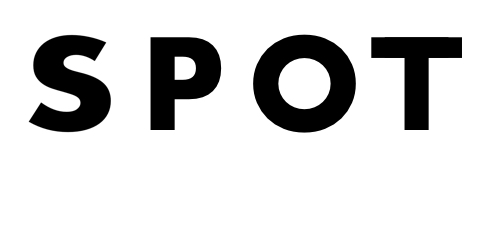
\includegraphics[width=0.6\linewidth]{figures/spot.pdf}
        \caption{%
            Time evolution of a Gaussian absorption line on a rigidly rotating, spotted star computed from the analytic formulae in \S\ref{sec:kT}.
            The stellar surface is modeled as a spherical harmonic expansion up to $l_\mathrm{max}=20$, and the line shape is assumed to be the same everywhere;
            the spot simply downweights the local intensity at all wavelengths.
            As the spot rotates into view (left panel), the line shape changes slightly (center panel). 
            The residuals between the line when the spot is in view (solid) and when it is on the backside of the star (dotted) are shown in the right panel, where a Gaussian-like feature can be seen tracking the spot as it rotates from the blueshifted hemisphere to the redshifted hemisphere of the star.
        }
        \label{fig:spot}
    \end{centering}
\end{figure}

Figure~\ref{fig:compare} shows one of the spectra in Figure~\ref{fig:spot}, this time computed using both our formulae (blue line) and the traditional technique of discretizing the stellar surface, Doppler-shifting the spectrum in each grid cell according to the local radial velocity, interpolating back to a uniform wavelength grid, and summing over the spatial dimension (dotted orange line). 
We show the residuals in the lower panel, where it is clear that as the number of grid cells increases from $10^2$ (light grey) to $10^5$ (dark grey), the numerical solution approaches the solution obtained using our approach.

%Understand---and comment on---the fundamental
%differences between a discrete linear convolution and traditional linear 
%interpolation. 
%Should we expect the numerical solution to actually \emph{converge}
%to the \starry solution, or is the way the two are interpolating fundamentally
%different?

\begin{figure}[t!]
    \begin{centering}
        \includegraphics[width=0.65\linewidth]{figures/compare.pdf}
        \caption{%
            The observed spectrum when the spot is in view computed with
            \starry (blue) and numerically (orange). 
            The problem setup is the same as that in Figure~\ref{fig:spot}. 
            The bottom panel shows the absolute value of the difference between the two spectra for different number of grid points in the numerical solution.
            As the number of grid points increases, the numerical solution approaches the \starry solution.
        }
        \label{fig:compare}
    \end{centering}
\end{figure}

\section{Linearization}
\label{sec:linear}

\begin{figure}[ht!]
    \begin{centering}
        \includegraphics[width=0.8\linewidth]{figures/linalg.pdf}
        \caption{%
            The Doppler design matrix $\Doppler$ (Equation~\ref{eq:linear:f}), constructed from a grid of Toeplitz matrices, each of shape $K \times K'$, where $K$ is the number of wavelength bins in the observed spectrum and $K' = K + W - 1$ is the number of bins in the model spectrum, where $W$ is the width of the convolution kernel.
            The $N$ columns of $\Doppler$ correspond to the Toeplitz matrices for each of the $N$ spherical harmonics (shown at the top);
            the $M$ rows correspond to the Toeplitz matrices rotated to each of the $M$ stellar phases observed (indicated graphically to the left of $\Doppler$).
        }
        \label{fig:linalg}
    \end{centering}
\end{figure}

Although the convolution operator (Equation~\ref{eq:deconv:convolution_def})
is defined for continuous functions, the problem of Doppler imaging deals with discrete measurements of a spectrum in bins of log wavelength. 
Provided our wavelength grid is fine enough, we may therefore approximate Equation~(\ref{eq:deconv:convolution_def}) with a discrete convolution.
For discrete arrays $\bvec{g}$ and $\bvec{h}$, we have
%
\begin{align}
    \label{eq:linear:convolution_def}
    \bvec{g} * \bvec{h} = \bvec{T(g)} \, \bvec{h}
\end{align}
%
where $\bvec{T}$ is a Toeplitz matrix, a matrix whose diagonals are constant from top left to bottom right. 
In this case, the diagonals are constructed from the values of $\bvec{g}$. 
If $\bvec{g}$ has length $L$, element $g_n$ is placed everywhere along the $k^\mathrm{th}$ diagonal of $\bvec{T}$ for $k = -L / 2 + n$; all other entries of $\bvec{T}$ are set to zero. 
Note that the matrix $\bvec{T}$ need not be square; in fact, for our purposes, it is a $(K \times K')$ matrix, where $K$ is the size of the observed wavelength grid and $K' = K + W - 1$ is the size of the wavelength grid in the rest frame, where $W$ is the width of the convolution kernel.

Given this formulation, we may re-write Equation~(\ref{eq:deconv:F}) as a purely linear operation on $\alm(\lnlam_0)$:
%
\begin{align}
    \label{eq:linear:ft}
    \bvec{f}_m
     & =
    \Doppler_m
    \,
    \alm
    \quad,
\end{align}
%
where $\Doppler_m$ is a $(K \times N K')$ matrix constructed by horizontally concatenating the Toeplitz matrices for each of the $N$ components of the convolution kernel $\kT(\lnlam)$ transformed by the rotation matrix $\bvec{R}(t)$ evaluated at time $t = t_m$:
%
\begin{align}
    \label{eq:linear:Dm}
    \Doppler_m =
    \begin{pmatrix}
        \bvec{T}(\kT_0)
        \quad
         &
        \quad
        \bvec{T}(\kT_1)
        \quad
         &
        \quad
        \cdots
        \quad
         &
        \quad
        \bvec{T}(\kT_N)
        \quad
    \end{pmatrix}
    (\bvec{R}(t_m) \otimes \bvec{I}_{K'})
    \quad.
\end{align}
%
where $\bvec{I}_{K'}$ is the $(K' \times K')$ identity matrix and $\otimes$ denotes the Kronecker product.
%
The $(K \times 1)$ vector $\mathbf{f}_m$ is the model for the flux observed at each wavelength at time $t = t_m$, and the $(N K' \times 1)$ vector $\alm$ is the vector representation of the spatially-dependent spectrum of the star. 
The latter is constructed by flattening the spherical harmonic expansion of the star such that the first $K'$ terms in $\alm$ correspond to the the values of $a_{0,0}$ at each wavelength $\lnlam_0$, followed by the values of $a_{1,-1}$ at each wavelength, and so forth.

In general, our data will consist of observations made at several epochs, corresponding to different rotational phases of the star.
If we concatenate all $M$ spectra $\bvec{f}_m$ into the $(MK \times 1)$ vector $\bvec{f}$, we may write
%
\begin{align}
    \label{eq:linear:f}
    \bvec{f}
     & =
    \Doppler
    \,
    \alm
    \quad,
\end{align}
%
where $\Doppler$ is the full $(MK \times N K')$ Doppler design matrix, constructed by vertically concatenating the individual matrices $\Doppler_m$:
%
%
\begin{align}
    \label{eq:linear:D}
    \Doppler =
    \begin{pmatrix}
        \Doppler_0
        \\
        \Doppler_1
        \\
        \cdots
        \\
        \Doppler_m
    \end{pmatrix}
    \quad.
\end{align}
%
%
Equation~(\ref{eq:linear:f}) represents the full linearization of the problem, where we have expressed the quantity we can observe, $\bvec{f}$, as a linear operation on the quantity of interest, the spectral/spatial decomposition of the stellar surface, $\alm$. 
Figure~\ref{fig:linalg} shows an example of $\Doppler$.

\section{The inverse problem}
\label{sec:inverse}
%
In the previous section we showed how to express the data vector $\bvec{f}$, a series of spectra obtained at different epochs, as a purely linear operation on the map vector $\alm$, the spherical harmonic decomposition of the specific intensity on the surface of the star. 
The advantage of this linearity is that, given suitable priors, it allows one to compute both the maximum likelihood solution for $\alm$ and its uncertainty \emph{analytically}. 
In particular, if one places a (multidimensional) Gaussian prior on $\alm$ with mean $\boldsymbol{\mu}_\mathbf{a}$ and covariance $\boldsymbol{\Lambda}_\mathbf{a}$, the maximum \emph{a posteriori} (MAP)
solution for $\alm$ is
%
\begin{align}
    \label{eq:inverse:ahat}
    \bvec{\hat{a}} & =
    \boldsymbol{\Sigma}_\mathbf{\hat{a}}
    \left(
    \Doppler^\top
    {\boldsymbol{\Sigma}_\mathbf{f}}^{-1}
    \bvec{f}
    +
    {\boldsymbol{\Lambda}_{\alm}}^{-1} \boldsymbol{\mu}_\mathbf{a}
    \right)
    \quad,
\end{align}
%
with posterior covariance given by
%
\begin{align}
    \label{eq:inverse:acov}
    \boldsymbol{\Sigma}_\mathbf{\hat{a}} & =
    \left(
    \Doppler^\top
    {\boldsymbol{\Sigma}_\mathbf{f}}^{-1}
    \Doppler
    +
    {\boldsymbol{\Lambda}_{\alm}}^{-1}
    \right)^{-1}
    \quad,
\end{align}
%
where $\boldsymbol{\Sigma}_\mathbf{f}$ is the data covariance matrix. 
These equations require the inversion of a few fairly large matrices, but as we will see later, it allows one to obtain the map of the star ($\bvec{\hat{a}}$) and its uncertainty ($\boldsymbol{\Sigma}_{\mathbf{\hat{a}}}$) in under a second for a typical dataset.

There is, however, a catch: for most practical purposes, it is difficult to find a good Gaussian prior for $\bvec{a}$. 
Usually we will have some prior information on what the spectrum of the star is, and perhaps some prior information on the distribution of surface features such as starspots. 
The problem is that even if these priors are Gaussian, the corresponding prior on $\bvec{a}$ is \emph{not}. 
To understand this, consider the case where the stellar rest frame spectrum is spatially constant, save for an amplitude that is spatially variable. 
We can then describe the rest frame spectrum by the $(K' \times 1)$ vector $\bvec{s}$ and the amplitude by the $(N \times 1)$ vector $\bvec{y}$ representing the spherical harmonic expansion of the intensity profile of the star. 
The vector $\alm$ is then given by the (flattened) outer product of the two vectors:
%
\begin{align}
    \label{eq:inverse:alm}
    \alm & = \mathrm{vec}\left( \bvec{A} \right) \nonumber             \\
           & = \mathrm{vec}\left( \bvec{s} \, \bvec{y}^\top \right) \quad,
\end{align}
%
where $\mathrm{vec}$ denotes the vectorization operation, which in this case transforms the $(K' \times N)$ matrix $\bvec{A}$ into the $(N K' \times 1)$ column vector $\alm$ by vertically stacking all of its columns. 
In other words, the vector $\alm$ consists of the set of $K'$ intensities in each wavelength bin repeated $N$ times, each time multiplied by the $n^\mathrm{th}$ spherical harmonic coefficient in the expansion of the surface intensity. 
Returning to our point about priors, note that all of the entries of $\alm$ are the product of two independent random variables. 
Since the product of two random variables is generally non-Gaussian, even when the variables themselves are Gaussian%
\footnote{see, e.g., \url{http://mathworld.wolfram.com/NormalProductDistribution.html}}%
, so too is the prior on $\alm$. 
This point makes Equation~(\ref{eq:inverse:ahat}) tricky to use in practice, since a multivariate Gaussian is not generally the most suitable prior for $\alm$.

That said, a Gaussian prior \emph{is} typically suitable for both the spectrum $\bvec{s}$ and the intensity $\bvec{y}$ (just not their product). 
It is straightforward to show that because Equation~(\ref{eq:linear:f}) is linear in $\alm$, it is also linear in both $\bvec{s}$ and $\bvec{y}$, so MAP solutions can be found analytically for $\bvec{s}$ (conditioned on $\bvec{y}$) and $\bvec{y}$ (conditioned on $\bvec{s}$). 
We investigate these solutions below.

\subsection{Solution for the map}
\label{sec:solve_y}
%
For a fixed, spatially constant rest-frame spectrum $\bvec{s}$, the model for the flux vector may be written as
%
\begin{align}
    \label{eq:inverse:fy}
    \bvec{f}
     & =
    \Doppler
    \,
    \bvec{S}
    \,
    \bvec{y}
    \quad,
\end{align}
%
where
%
\begin{align}
    \label{eq:inverse:S}
    \bvec{S} =
    \begin{pmatrix}
        \quadquad\bvec{s}\quadquad &                            &                            &                            &        \\
                                   & \quadquad\bvec{s}\quadquad &                            &                            &        \\
                                   &                            & \quadquad\bvec{s}\quadquad &                            &        \\
                                   &                            &                            & \quadquad\bvec{s}\quadquad &        \\
                                   &                            &                            &                            & \ddots
    \end{pmatrix}
\end{align}
%
is a $(NK' \times N)$ block matrix constructed by repeating the column vector $\bvec{s}$ $N$ times in blocks along the main diagonal.
%
Given prior mean $\boldsymbol{\mu}_\bvec{y}$ and covariance $\boldsymbol{\Lambda}_\bvec{y}$ on $\bvec{y}$, the MAP solution is given by
%
\begin{align}
    \label{eq:inverse:y1hat}
    \bvec{\hat{y}} & =
    \boldsymbol{\Sigma}_\mathbf{\hat{y}}
    \left(
    \bvec{S}^\top\Doppler^\top
    {\boldsymbol{\Sigma}_\mathbf{f}}^{-1}
    \bvec{f}
    +
    {\boldsymbol{\Lambda}_\bvec{y}}^{-1} \boldsymbol{\mu}_\bvec{y}
    \right)
    \quad,
\end{align}
%
with covariance
%
\begin{align}
    \label{eq:inverse:y1cov}
    \boldsymbol{\Sigma}_\bvec{\hat{y}} & =
    \left(
    \bvec{S}^\top\Doppler^\top
    {\boldsymbol{\Sigma}_\bvec{f}}^{-1}
    \Doppler\bvec{S}
    +
    {\boldsymbol{\Lambda}_\bvec{y}}^{-1}
    \right)^{-1}
    \quad.
\end{align}
%
If we choose a prior with zero mean ($\boldsymbol{\mu}_\bvec{y} = 0$)
and a diagonal covariance that is constant for each spherical harmonic order $m$,
%
\begin{align}
    \boldsymbol{\Lambda}_\bvec{y} & =
    \mathrm{diag} \left(
    \sigma_0^2
    \quad\quad\quad\quad
    \sigma_1^2
    \quad\quad\quad\quad
    \sigma_1^2
    \quad\quad\quad\quad
    \sigma_1^2
    \quad\quad\quad\quad
    \sigma_2^2
    \quad\quad\quad\quad
    \sigma_2^2
    \quad\quad\quad\quad
    \sigma_2^2
    \quad\quad\quad\quad
    \sigma_2^2
    \quad\quad\quad\quad
    \sigma_2^2
    \quad\quad\quad\quad
    \cdots
    \right)
    \quad,
\end{align}
%
we are in fact imposing an isotropic prior with an angular power spectrum given by $C_l = \sigma_l^2$
\citep[e.g.,][]{Baldi2006}. 
This is especially useful if the typical angular scale of features on the surface of the star is known or if a Gaussian prior can be placed on it.

\subsection{Solution for the spectrum}
\label{sec:solve_s}
%
If, on the other hand, the spatial intensity profile is known, the model for the flux vector may be written in terms of the spectrum $\bvec{s}$ as
%
\begin{align}
    \label{eq:inverse:fs}
    \bvec{f}
     & =
    \Doppler
    \,
    \bvec{Y}
    \,
    \bvec{s}
    \quad,
\end{align}
%
where
%
\begin{align}
    \label{eq:inverse:Y}
    \bvec{Y} =
    \begin{pmatrix}
        y_{0,0}\, \bvec{I}_{K'} \\
        y_{1,-1}\, \bvec{I}_{K'} \\
        y_{1,0}\, \bvec{I}_{K'} \\
        y_{1,1}\, \bvec{I}_{K'} \\
        \cdots
    \end{pmatrix}
\end{align}
%
is a $(NK' \times K')$ matrix constructed by vertically stacking $N$ $(K' \times K')$ identity matrices, each multiplied by the corresponding coefficient of $\bvec{y}$. 
Given prior mean $\boldsymbol{\mu}_\mathbf{s}$ and covariance $\boldsymbol{\Lambda}_\mathbf{s}$ on $\mathbf{s}$, the MAP solution is given by
%
\begin{align}
    \label{eq:inverse:shat}
    \bvec{\hat{s}} & =
    \boldsymbol{\Sigma}_\mathbf{\hat{s}}
    \left(
    \bvec{Y}^\top\Doppler^\top
    {\boldsymbol{\Sigma}_\mathbf{f}}^{-1}
    \bvec{f}
    +
    {\boldsymbol{\Lambda}_\mathbf{s}}^{-1} \boldsymbol{\mu}_\mathbf{s}
    \right)
    \quad,
\end{align}
%
with covariance
%
\begin{align}
    \label{eq:inverse:scov}
    \boldsymbol{\Sigma}_\mathbf{\hat{s}} & =
    \left(
    \bvec{Y}^\top\Doppler^\top
    {\boldsymbol{\Sigma}_\mathbf{f}}^{-1}
    \Doppler\bvec{Y}
    +
    {\boldsymbol{\Lambda}_\mathbf{s}}^{-1}
    \right)^{-1}
    \quad.
\end{align}

\subsection{The full solution}
\label{sec:full_solve}
%
In the previous two sections we showed how, if the stellar rest-frame spectrum is spatially constant and known \emph{a priori} (from, say, a template spectrum), the posterior distribution for the surface map $\bvec{y}$ is \emph{analytic} (Equations~\ref{eq:inverse:y1hat} and \ref{eq:inverse:y1cov}). 
Conversely, if the surface map is known, the posterior for the spectrum is also analytic (Equations~\ref{eq:inverse:shat} and \ref{eq:inverse:scov}). 
Both sets of solutions require Gaussian priors on the quantities of interest, but these are easily interpretable. 
A Gaussian prior on the spherical harmonic coefficients of the surface map corresponds to the angular power spectrum of the surface features, whereas a Gaussian prior on the spectrum can be used to correctly propagate uncertainties in the stellar spectrum from observational uncertainties on the stellar metallicity, temperature, etc.

Importantly, the framework developed here allows one to analytically compute not only the ``optimal'' solution to the Doppler imaging problem, but also its uncertainty. 
The problem of re-constructing surface images of stars from spectra and/or light curves is fundamentally ill-posed because of intrinsic degeneracies and a large null space \citep[e.g.,][]{Cowan2017,Luger2019}. 
Coupled to uncertainties in the observations themselves, this makes the process of searching for the ``optimal'' solution flawed at best, and meaningless at worst. 
Access to the full covariance matrix of the solution is therefore essential to assessing our confidence in the various features of the inferred surface maps.

However, as we mentioned above, the Doppler imaging problem can be solved analytically for either the surface map or the spectrum, but not typically both. 
If neither are known exactly \emph{a priori}, which is quite often the case, we can still find the MAP solution quickly by guessing at an initial spectrum $\bvec{s}$ and iterating between optimizing for $\bvec{y}$ and optimizing for $\bvec{s}$. 
This bilinear problem is not generally convex, but given a good starting point for $\bvec{s}$ and sufficient regularization on $\bvec{y}$, we find that it typically converges to the correct solution, especially after refinement with a nonlinear solver; we discuss this in detail below.

Once the MAP solution has been found for both $\bvec{s}$ and $\bvec{y}$, the covariance of one conditioned on the other can be computed from the formulae above. 
However, this is necessarily a lower bound on the true covariance of the solution, since it neglects any covariance \emph{between} $\bvec{s}$ and $\bvec{y}$. 
To \emph{correctly} account for this, one must resort to Monte Carlo methods or other sampling techniques. 
We discuss this further below.

\section{Further considerations}
\label{sec:bellswhistles}
%
Before we demonstrate our formalism in practice, we consider three modifications to our model that are often required when modeling real data. 
Below we discuss what to do when the relative brightness of the star across different observations is unknown (\S\ref{sec:norm}), how to account for the effects of limb darkening (\S\ref{sec:ld}), and how to model stars whose local spectra differ within and outside of starspots (\S\ref{sec:eigen}).

\subsection{Unknown continuum normalization}
\label{sec:norm}
%
Consider the star depicted in Figure~\ref{fig:spot}. 
When the spot is in view, absorption lines become distorted due to the suppression of either blueshifted or redshifted light. 
However, what is not shown in the figure is the fact that overall, the star also gets \emph{dimmer}: the continuum level drops in the presence of the spot. 
Unfortunately, spectrographs are not usually designed to measure this, since the change in the star's overall brightness from one observation to the next is often dwarfed by (unknown) changes in the spectrograph sensitivity, cloud cover, etc.
For this reason, the spectra are usually normalized to have a fixed baseline continuum, and Equation~\ref{eq:linear:f} is no longer a good model for the data.

One option is to collect simultaneous photometry on the target in a band similar to the wavelength range observed, and use this light curve to (un-)normalize the spectral timeseries $\bvec{f}$. 
However, when this is not an option, our model for $\bvec{f}$ (Equation~\ref{eq:linear:f}) must be amended:
%
\begin{align}
    \label{eq:norm:f}
    \fnorm
     & =
     \frac{
        \mathbf{f}
    } {
        \bvec{B}
        \,
        \alm
    }
    \nonumber 
    \\[1em]
    & =
    \frac{
        \Doppler
        \,
        \alm
    } {
        \bvec{B}
        \,
        \alm
    }
    \quad,
\end{align}
%
where $\fnorm$ is the normalized spectral timeseries,
$\bvec{B}$ is the baseline design matrix, and the vector division is performed
elementwise. 
If $c$ is an index in the observed spectrum corresponding to the continuum (at all epochs), the elements of $\bvec{B}$ are computed from
%
\begin{align}
    B_{ij} = D_{i'j}
\end{align}
%
where
%
\begin{align}
    i' = c + \bigg\lfloor\frac{i}{K}\bigg\rfloor K
    \quad.
\end{align}
%
In other words, the matrix $\bvec{B}$ is constructed by repeating the $c^\mathrm{th}$ row of each epoch block $\Doppler_m$ of $\Doppler$ $K$ times.
Equation~(\ref{eq:norm:f}) is therefore equivalent to computing the $M$ unnormalized spectra using Equation~(\ref{eq:linear:f}) and dividing each one by the value at index $c$.


Given this new equation, we must change how we approach the inverse problem (\S\ref{sec:inverse}) if our data vector is the normalized spectral timeseries $\fnorm$. 
When solving for the spectrum given the spherical harmonic vector (\S\ref{sec:solve_s}), we need only make the replacements 
$\bvec{f} \rightarrow \fnorm \circ (\bvec{B}\, \bvec{a})$ 
and 
$\boldsymbol{\Sigma}_\mathbf{f} \rightarrow \boldsymbol{\Sigma}_{\fnorm} \circ (\bvec{B}\, \bvec{a})^2$ 
in Equations~(\ref{eq:inverse:shat}) and (\ref{eq:inverse:scov}), where $\circ$ denotes the elementwise product.
However, when solving for the spherical harmonic vector given the spectrum (\ref{sec:solve_y}), the problem is no longer linear in $\bvec{y}$, as the vector of interest appears in both the numerator and the denominator:
%
\begin{align}
    \label{eq:norm:fy}
    \fnorm
     & =
    \frac{
        \bvec{D}
        \,
        \bvec{S}
        \,
        \bvec{y}
    }{
        \bvec{B}
        \,
        \bvec{S}
        \,
        \bvec{y}
    }
    \quad.
\end{align}
%
Unfortunately, this equation does not admit a closed form solution for $\mathbf{y}$. 
One can, however, still solve for the maximum a posteriori value of $\mathbf{y}$ in an efficient manner by iteratively solving for the baseline and then for the spherical harmonic coefficients.
We describe a procedure for this in \S\ref{sec:spotstar} below.

\subsection{Limb darkening}
\label{sec:ld}
%
Thus far we have avoided mention of limb darkening, whose effect on the observed spectrum can often be significant. 
A proper treatment of limb darkening requires solution of radiative transfer equations and should account for the temperature and composition gradients in the stellar atmosphere. 
However, in the spirit of data-driven inference, we can approximate the effect of limb darkening by weighting the spatial component of our map by the limb darkening profile of the star, which can either be imposed or learned from the data. 
For a polynomial limb darkening law of the form
%
\begin{align}
    \label{eq:ld:I}
    \frac{I(\mu)}{I(\mu = 1)} = 1 - \sum_{n=1}^{n_\mathrm{max}} u_n(1 - \mu)^n
    \quad,
\end{align}
%
where $\mu = z = \sqrt{1 - x^2 - y^2}$ is the radial coordinate on the projected disk and $u_n$ is a limb darkening coefficient, the effect of limb darkening on the stellar map can be expressed exactly as a linear operation on the spherical harmonic coefficient vector \citep{Luger2019,Agol2020}. 
This can be understood by noting that all terms in Equation~(\ref{eq:ld:I}) are strictly polynomials in $x$, $y$, and $z$, all of which can be expressed exactly as sums of spherical harmonics \citep{Luger2019}. 
When weighting the surface intensity by the limb darkening profile, the resulting intensity is simply a product of spherical harmonics, which is itself a sum of spherical harmonics. 
Given a limb darkening law of degree $n_\mathrm{max}$, we can always construct a matrix $\bvec{L}$ that transforms a spherical harmonic vector $\bvec{y}$ of degree $l_\mathrm{max}$ to a limb-darkened spherical harmonic vector $\bvec{y'}$ of degree $l_\mathrm{max} + n_\mathrm{max}$. 
As an example, consider a map of degree $l_\mathrm{max} = 1$ and the linear limb darkening law ($n_\mathrm{max} = 1$).
The transformation matrix from $\bvec{y}$ to $\bvec{y'}$ is
%
\begin{align}
    \label{eq:ld:L}
    \bvec{L} =
    \frac{1}{1 - \frac{u_1}{3}}
    \begin{pmatrix}
        \quadquad1-u_1\quadquad & 0                       & \frac{u_1}{\sqrt{3}}    & 0                       \\
        0                       & \quadquad1-u_1\quadquad & 0                       & 0                       \\
        \frac{u_1}{\sqrt{3}}    & 0                       & \quadquad1-u_1\quadquad & 0                       \\
        0                       & 0                       & 0                       & \quadquad1-u_1\quadquad \\
        0                       & 0                       & 0                       & 0                       \\
        0                       & \frac{u_1}{\sqrt{5}}    & 0                       & 0                       \\
        0                       & 0                       & \frac{2u_1}{\sqrt{15}}  & 0                       \\
        0                       & 0                       & 0                       & \frac{u_1}{\sqrt{5}}    \\
        0                       & 0                       & 0                       & 0
    \end{pmatrix}
    \quad.
\end{align}
%
The columns of $\bvec{L}$ are constructed from the coefficient vectors of each transformed spherical harmonic, which are in turn computed by multiplying each spherical harmonic by the spherical harmonic decomposition of the particular limb darkening law.
Figure~\ref{fig:ld} shows this transformation with $u_1 = 1$ applied to each of the first four spherical harmonics.
%
\begin{figure}[t!]
    \begin{centering}
        \includegraphics[width=0.5\linewidth]{figures/ld.pdf}
        \caption{%
            Illustration of the limb darkening transformation given by Equation~(\ref{eq:ld:L}) for a linear limb darkening law with $u_1 = 1$. 
            Each row shows a spherical harmonic before (left) and after (right) transformation by $\bvec{L}$.
        }
        \label{fig:ld}
    \end{centering}
\end{figure}
%

Now, to incorporate limb darkening into our model, we must modify how we compute the Doppler design matrix $\Doppler$ (Equation~\ref{eq:linear:D} and Figure~\ref{fig:linalg}). 
Recall that this matrix is constructed by vertically stacking the submatrices $\Doppler_m$ given by Equation~(\ref{eq:linear:Dm}), which we now compute as
%
\begin{align}
    \label{eq:ld:Dm}
    \Doppler_m =
    \begin{pmatrix}
        \quad
        \bvec{T}(\kT_0)
        \quad
         &
        \quad
        \bvec{T}(\kT_1)
        \quad
         &
        \quad
        \cdots
        \quad
         &
        \quad
        \bvec{T}(\kT_{N'})
        \quad
    \end{pmatrix}
    (\bvec{L} \, \bvec{R}(t_m) \otimes \bvec{I}_{K'})
    \quad,
\end{align}
%
where we have replaced the rotation matrix $\bvec{R}(t_m)$ with the linear transformation $\bvec{L}\,\bvec{R}(t_m)$, which first rotates the input spherical harmonic coefficient vector to the correct phase then limb darkens it. 
Note also that the terms in the convolution kernel $\kT$ are now indexed from 0 to $N' = (l_\mathrm{max} + n_\mathrm{max} + 1)^2$, where $n_\mathrm{max}$ is the degree of the limb darkening operator.

Note that it is also possible to model wavelength-dependent limb darkening in this fashion. 
The procedure is similar, except that the limb darkening coefficients $u_n$ are now functions of $\lnlam$, and each element of the matrix $\bvec{L}$ is now a vector of length $K'$. 
The submatrices $\Doppler_m$ may be written as
%
\begin{align}
    \label{eq:ld:Dmwav}
    \resizebox{0.91\textwidth}{!}{
        $
            \Doppler_m =
            \begin{pmatrix}
                \quad
                \bvec{T}(\kT_0)
                \quad
                 &
                \quad
                \bvec{T}(\kT_1)
                \quad
                 &
                \quad
                \cdots
                \quad
                 &
                \quad
                \bvec{T}(\kT_{N'})
                \quad
            \end{pmatrix}
            \begin{pmatrix}
                \mathrm{diag}(\bvec{L}_{0,0})
                 &
                \mathrm{diag}(\bvec{L}_{0,1})
                 &
                \cdots
                 &
                \mathrm{diag}(\bvec{L}_{0,N})
                \\
                \mathrm{diag}(\bvec{L}_{1,0})
                 &
                \mathrm{diag}(\bvec{L}_{1,1})
                 &
                \cdots
                 &
                \mathrm{diag}(\bvec{L}_{1,N})
                \\
                \cdots
                 &
                \cdots
                 &
                \ddots
                 &
                \cdots
                \\
                \mathrm{diag}(\bvec{L}_{N',0})
                 &
                \mathrm{diag}(\bvec{L}_{N',1})
                 &
                \cdots
                 &
                \mathrm{diag}(\bvec{L}_{N',N})
            \end{pmatrix}
            (\bvec{R}(t_m) \otimes \bvec{I}_{K'})
        $
    }
    \quad,
\end{align}
%
where $\mathrm{diag}(\bvec{v})$ denotes the $(K' \times K')$ diagonal matrix constructed by placing the vector $\bvec{v}$ along the main diagonal.

\subsection{Multiple spectral components}
\label{sec:eigen}
%
In our discussion so far we have focused on the particular case where the spectral/spatial decomposition of the stellar surface can be expressed as the outer product of two vectors (Equation~\ref{eq:inverse:alm}). 
As we mentioned previously, this corresponds to the case where the spectrum is constant across the surface of the star except for a spatially-variable amplitude: i.e., spots have the same spectrum as the rest of the star, but emit less flux overall. 
However, most of the formalism developed here also applies to the more general case where the spectrum at a particular point on the surface of the star is a linear combination of several different spectral components. 
In this case, the map vector $\alm$ may be written as the sum over $J$ spectra $\bvec{s}_j$, each of which is dotted into a different vector of spherical harmonic coefficients $\bvec{y}_j^\top$:
%
\begin{align}
    \label{eq:eigen:alm}
    \alm
     & =
    \sum_{j=0}^{J-1}\mathrm{vec}\left( \bvec{s}_j \, \bvec{y}_j^\top \right) \\
     & =
    \mathrm{vec}\left( \boldsymbol{\mathbb{S}} \, \boldsymbol{\mathbb{Y}}^\top \right) \quad,
\end{align}
%
where $\boldsymbol{\mathbb{S}}$ is the $(K' \times J)$ matrix whose columns are the $J$ spectral components and $\boldsymbol{\mathbb{Y}}^\top$ is the $(J \times N)$ matrix whose rows are the corresponding $J$ spherical harmonic coefficient vectors.

The model remains linear in both the spherical harmonic coefficients and the spectral components, and the procedures outlined in \S\ref{sec:inverse} may still be followed to solve the inverse problem, provided we unroll these matrices into vectors, letting $\mathbf{s} = \mathrm{vec}(\boldsymbol{\mathbb{S}})$ and $\mathbf{y} = \mathrm{vec}(\boldsymbol{\mathbb{Y}})$.
We present an example of inference on a two-component stellar spectrum in \S\ref{sec:twospec}
below.

\section{Application to a spotted star}
\label{sec:spotstar}

In this section we apply the formalism developed in \S\ref{sec:inverse} and \S\ref{sec:bellswhistles} to a synthetic dataset of a rapidly rotating spotted star. 
This section is motivated by the examples in \cite{Vogt1987}, who generated rotationally-broadened spectra of a rapidly-rotating star with the letters ``VOGT'' painted across the northern hemisphere. 
In that paper, the authors generated synthetic line profiles of the Fe I $\lambda 6430$ absorption line with equivalent width $W \approx 10$~km/s and from these computed rotationally broadened spectra for a star at an inclination $i=40^\circ$ rotating at projected velocity $v\sin i = 40$~km/s.
The spectra were computed at 16 equally spaced rotational phases and downsampled to 32 wavelength bins per epoch, for a total of 512 data points.

\begin{figure}[t!]
    \begin{centering}
        \includegraphics[width=0.85\linewidth]{figures/spot_setup.pdf}
        \caption{%
            The basic setup for the \spot problem. 
            We compute the $l_\mathrm{max} = 15$ spherical harmonic expansion of a map where the word ``SPOT'' has been placed across the northern hemisphere (top left). 
            Each point on the surface is given the same spectrum, composed of a sum of synthetic Gaussian absorption lines (blue curve in the bottom panel).
            The specific intensity at each point on the surface is equal to this spectrum weighted by the intensity of the map, which is close to zero within the spot (point labeled \texttt{B}) and close ot unity outside the spot (point labeled \texttt{A}).
            To generate the synthetic dataset (orange curves in the bottom panel), the star is inclined at $40^\circ$ with respect to the line of sight and the disk-integrated spectrum is computed at 16 equally-spaced phases between $-180^\circ$ and $180^\circ$ (middle panel).
            The grey regions indicate wavelength regions outside the observation window, but whose features can still contribute to the observed spectrum due to rotational broadening.
        }
        \label{fig:spot_setup}
    \end{centering}
\end{figure}

We repeat the same experiment here using our new formalism, except we instead generate a stellar surface with the word ``SPOT'' written across the northern hemisphere (top left panel of Figure~\ref{fig:spot_setup}).
We do this by computing the $l_\mathrm{max} = 15$ spherical harmonic decomposition of an image of the word, generating a set of $N = (l_\mathrm{max} + 1)^2 = 256$ spherical harmonic coefficients $\bvec{y}$. 
We assume an equatorial velocity $v = 60$ km/s and an inclination $i = 40^\circ$, such that $v \sin i = 38.6$~km/s (compare to $i = 40^\circ$ and $v \sin i = 40$~km/s in \citealt{Vogt1987}).

Our input spectrum $\bvec{s}$ was generated at high resolution ($R \equiv \frac{\lambda}{\Delta\lambda} = 430,000$) centered on the Fe I $\lambda 6430$ absorption line (blue curve in the bottom panel of Figure~\ref{fig:spot_setup}).
%
The spectrum consists of a (purely synthetic) Gaussian absorption line of fractional depth 50\% centered at $\lambda = 643$~nm with FWHM of $0.02$~nm, or, in velocity space, $\Delta v = \mathrm{FWHM} \times c / \lambda \approx~10$~km/s, equal to the value used in \citet{Vogt1987}. 
%
Unlike \citet{Vogt1987}, we add 20 additional small absorption lines at random positions throughout the spectrum, all of the same FWHM but of varying depths, including some line blends. 
In total, the rest frame spectrum $\bvec{s}$ consists of $K = 200$ wavelength bins in the range $642.85~\mathrm{nm} \leq \lambda \leq 643.15~\mathrm{nm}$ plus an additional
%
\begin{align}
    W & = 2 \bigg\lceil \frac{(v\sin i)_\mathrm{max}R}{c} \bigg\rceil \nonumber  \\
      & = 144
\end{align}
%
bins of padding (72 on either side) to eliminate edge effects due to the convolution, for a total of $K' = 344$ wavelength bins. 
In the expression above, $(v\sin i)_\mathrm{max}$ is the maximum value of $v\sin i$ we can model with a given value of $W$; for this experiment, we set $(v\sin i)_\mathrm{max}=50$~km/s, which is larger than the actual value of $v\sin i$ we used to generate the data (see above).
Finally, we linearly interpolate this spectrum to a wavelength grid uniform in log space to obtain the vector $\bvec{s}$ evaluated at each $\lnlam$.

Given $\bvec{y}$ and $\bvec{s}$, we use Equations~(\ref{eq:deconv:F}) and~(\ref{eq:inverse:alm}) to compute the data vector $\bvec{f}$ at $M = 16$ equally spaced rotational phases; these phases are shown in orthographic projection (as an observer would see the star) in the center panel of Figure~\ref{fig:spot_setup}. 
The synthetic spectra for each phase are shown as the orange curves in the bottom panel of the figure (note the different scaling, as all spectral lines become shallower due to the broadening). 
We assume a wavelength-independent, quadratic limb darkening law with $u_1 = 0.5$ and $u_2 = 0.25$. 
Finally, we divide the flux by the baseline at each epoch (Equation~\ref{eq:norm:f}) and add random Gaussian noise with amplitude $\sigma_\bvec{f} = 10^{-4}$ to simulate a very high signal-to-noise ratio (SNR) spectrum. 
The mean standard deviation in each wavelength bin across all 16 epochs in the noiseless data vector is about $10^{-2}$, so our choice of $\sigma_\bvec{f}$ corresponds to SNR $\sim$ 100 in each of the 200 wavelength bins of $\bvec{f}$.

%For reference, \citet{Vogt1987} report SNRs per 60 m\AA\, pixel, while our
%resolution elements are approximately $\lambda_r\Delta\lnlam/K \approx 100$ m\AA\,
%across, so our SNR in the same units as \citet{Vogt1987} is about 80.
%
% TODO: Perhaps Vogt computes the "signal" as the line depth, rather than
% as the amplitude of the perturbations? Check this.
% We Recover images with an effective resolution of $12^\circ$.

In the following sections we discuss various approaches to solving the Doppler imaging problem for this dataset.
Unless otherwise noted, in all experiments we adopt a Gaussian prior for the spherical harmonic coefficients $\bvec{y}$ with mean $\boldsymbol{\mu}_\bvec{y} = \bvec{0}$ and covariance $\boldsymbol{\Lambda}_\bvec{y}$, with
%
\begin{align}
    \label{eq:Lambday}
    {\Lambda_\bvec{y}}_{i, j} 
    =
    \begin{cases}
        1 & \quad\quad\quad\quad i = j = 0
        \\
        10^{-4}\delta_{ij} & \quad\quad\quad\quad \mathrm{otherwise}
        \quad,
    \end{cases}
\end{align}
%
corresponding to a flat power spectrum prior.
We also place a Gaussian prior on the spectrum $\bvec{s}$ with unit mean and covariance $\boldsymbol{\Lambda}_\bvec{s} = (10^{-1})^2\bvec{I}$.

\subsection{Known baseline and spectrum}
\label{sec:spot_y1}
%
In our first experiment, we attempt to infer the stellar map assuming we have perfect knowledge of the rest frame spectrum $\bvec{s}$ and the baseline.
This is analogous to the case where a good physical model exists for the stellar spectrum and simultaneous photometry is available to constrain the baseline variations.
As we showed in \S\ref{sec:solve_y}, the posterior distribution for the map coefficients $\bvec{y}$ is analytic in this case, with mean given by Equation~(\ref{eq:inverse:y1hat})
and covariance given by Equation~(\ref{eq:inverse:y1cov}). 
Note that we must first scale the data vector $\fnorm$ by the baseline (which in this case is known) to obtain $\bvec{f}$.

\begin{figure}[p!]
    \begin{centering}
        \includegraphics[width=0.39\linewidth]{figures/spot_infer_y_timeseries.pdf}
        \includegraphics[width=0.59\linewidth]{figures/spot_infer_y_maps.pdf}
        \caption{%
            The solution to the \spot problem at high SNR when both the rest frame spectrum and the baseline are known.
            The panel on the left shows the inferred map at each of the 16
            epochs, alongside the observed spectrum (black points) and the best-fit model (orange lines). 
            The Mollweide projection of the original map is shown at the top right; the inferred map is displayed below it. 
            The bottom panel shows the posterior uncertainty on the inferred intensity, ranging from close to zero in the northern hemisphere to $\sigma_\mathrm{prior} \approx 13\%$ below a latitude of $-30^\circ$. 
            The latter is the uncertainty associated with our particular choice of prior, as the southernmost latitudes of the star are never visible to the observer.
        }
        \label{fig:spot_infer_y}
    \end{centering}
\end{figure}

The results are shown in Figure~\ref{fig:spot_infer_y}. 
The left hand panel shows the inferred map alongside the data (black points) and best fit model (orange curves) at each of the 16 epochs.
The panels on the right show the true map (top), the inferred map (center)
and the posterior pointwise uncertainty (bottom) on a rectangular latitude-longitude grid. 
The uncertainty on the vector of pixels $\bvec{p}$ where we evaluate the map is equal to the square root of the diagonal of the posterior covariance matrix for the pixel values, computed from
%
\begin{align}
    \label{eq:spotstar:uncert}
    \boldsymbol{\Sigma}_\bvec{p} = \bvec{P} \boldsymbol{\Sigma}_\bvec{\hat{y}}\bvec{P}^\top
\end{align}
%
where $\bvec{P}$ is the change-of-basis matrix from spherical harmonic coefficients to pixels on the grid.

The inferred map is nearly indistinguishable from the true map, save for a few small differences, particularly below the stellar equator. 
This is captured by the uncertainty, which increases south of $+30^\circ$ latitude, reaching a maximum at $-30^\circ$, below which the uncertainty is constant at about 13\%. 
This is due to the fact that regions below $-40^\circ$ latitude are never in view from the observer's perspective, while regions between about $-30^\circ$ and $-40^\circ$ are so strongly limb-darkened that the data contains little information about them. 
The particular value of the uncertainty in this region---13\%---is the uncertainty associated with our choice of prior (Equation~\ref{eq:Lambday}).

\xxx{WORK IN PROGRESS BELOW THIS LINE}

\subsection{Known spectrum, unknown baseline}
\label{sec:spot_y1b}
%
We next investigate the case where the spectrum is known exactly, but the baseline is not. 
This corresponds to the case discussed in
\S\ref{sec:norm}. 
We use the solution to the linearized problem, Equation~(\ref{eq:norm:yhat}), to obtain an initial guess for $\bvec{y_1}$. 
We then repeatedly solve Equation~(\ref{eq:inverse:y1hat}) for $\bvec{y_1}$, given the baseline computed from the previous value of $\bvec{y_1}$ from Equation~(\ref{eq:norm:b}).
Because of the high SNR of our data, we find that it is necessary to employ a simple tempering procedure to avoid getting stuck in local minima. 
We introduce an artificial temperature $T$ that decreases every iteration in equally spaced logarithmic steps $\Delta \log T$ from an initial temperature $T=T_0$ to $T=1$. 
This temperature is used to scale the data covariance $\boldsymbol{\Sigma}_\bvec{f}$; in practice, we simply replace $\boldsymbol{\Sigma}_\bvec{f}$ with $T \boldsymbol{\Sigma}_\bvec{f}$ in Equation~(\ref{eq:inverse:y1hat}). 
This has the effect of smoothing out the likelihood space, reducing the likelihood that the solver will get stuck in a local minimum. 
For this particular experiment, we set $T_0 = 100$ and $\Delta \log T = -0.25$, for a total of $9$ steps of the bilinear solver.
%
In a final step, we run a gradient-descent optimizer, initializing it at the solution obtained with the bilinear solver. 
We use the \texttt{Keras} \citep{Keras} implementation of the Nesterov momentum-enhanced Adam solver \citep[\texttt{NAdam};][]{NAdam}, running it for $N_\mathrm{nadam} = 80$ iterations at a learning rate $L_\mathrm{nadam} = 10^{-4}$. 
Our loss function is simply the (negative) log probability, equal to the sum of the log likelihood and log prior:
%
\begin{align}
    \label{eq:spotstar:logP}
    -\ln P & =
    \frac{1}{2}
    \Big(
    \bvec{r}^\top \boldsymbol{\Sigma}_\bvec{f}^{-1} \bvec{r} \, + \,
    \bvec{y_1}^\top \boldsymbol{\Lambda}_\bvec{y_1}^{-1} \bvec{y_1} \, + \, (\bvec{b - 1})^\top \boldsymbol{\Lambda}_\bvec{b}^{-1} (\bvec{b - 1})
    \Big)
\end{align}
%
where $\bvec{r}$ is the residual (data minus model) vector and the last term is a prior we include on the baseline $\bvec{b}$, which we force to be close to a mean of unity with covariance $\boldsymbol{\Lambda}_\bvec{b} = (0.1)^2\bvec{I}$.

% \begin{figure}[p!]
%     \begin{centering}
%         \includegraphics[width=0.49\linewidth]{figures/spot_y1b_timeseries.pdf.pdf}
%         \includegraphics[width=0.49\linewidth]{figures/spot_y1b_rect.pdf}
%         \\[0.5em]
%         \includegraphics[width=0.405\linewidth]{figures/spot_y1b_baseline.pdf}
%         \includegraphics[width=0.575\linewidth]{figures/spot_y1b_coeffs.pdf}
%         \caption{%
%             Similar to Figure~\ref{fig:spot_y1}, but assuming the baseline is not known. 
%             The panel at the bottom left shows the true baseline (blue) and the inferred baseline (orange), along with its $1\sigma$ uncertainty. 
%             The large offset between the two highlights one of the fundamental degeneracies of the problem: since most of the southern hemisphere of the star is never visible, the coefficient of the $Y_{1,-1}$ (\raisebox{-0.2em}{\includegraphics[width=1em]{Y1m1.pdf}}) spherical harmonic is not constrained by the data, resulting in an unknowable additive offset in the baseline.
%             This effect can be seen also in (\emph{a}) the inferred map, where the background intensity in the northern hemisphere is significantly larger than that in the southern hemisphere, and (\emph{b}) the spherical harmonic coefficients (bottom right), where a large discrepancy is visible between the true and inferred values of the first two coefficients.
%         }
%         \label{fig:spot_y1b}
%     \end{centering}
% \end{figure}

Our results are shown in Figure~\ref{fig:spot_y1b}. 
The panels at the top are the same as those in Figure~\ref{fig:spot_y1}, but now we also plot the inferred baseline (lower left) and spherical harmonic coefficients (lower right) next to the true values. 
We recover the \texttt{SPOT} map just as well as before, except for the presence of a strong dipolar artifact; the background intensity level is higher in the northern hemisphere and lower in the southern hemisphere. 
This effect is closely related to the fact that we do not know the true baseline. 
While we are able to infer the shape of the baseline exceedingly well (lower left panel), there is a large offset between the true value and our inferred value. 
This is due to a fundamental degeneracy involving the $Y_{1,-1}$ (\raisebox{-0.2em}{\includegraphics[width=1em]{figures/Y1m1.pdf}}) spherical harmonic coefficient, which, because a large portion of the southern hemisphere is never in view, cannot be constrained by the data. 
The magnitude of the true value of the coefficient is quite large (lower right panel), since the northern hemisphere \emph{is} significantly darker than the southern hemisphere; however, the data do not constrain this, and our prior shrinks all coefficients toward zero. 
The net effect is that the region surrounding the spot in the northern hemisphere gets brighter to even out the difference between the two hemispheres. 
This causes the visible portion of the star to get brighter, raising the baseline relative to the true value.

Note, importantly, that even in cases where the baseline is known (from, say, simultaneous photometry), it is typically only known in a \emph{relative} sense. 
This degeneracy will typically apply in that case as well, so in principle the dipole term will always be unconstrained for stars at similar inclinations. 
For inclinations closer to $90^\circ$ this is much less of an issue, although (as we will see below) other degeneracies show up.

Finally, we note that the pixelwise uncertainty shown is a strict \emph{lower bound} on the map uncertainty, since it is the uncertainty conditioned on the inferred value of the baseline. 
Sampling methods such as MCMC are required to obtain the \emph{true} uncertainty on the map. 
We discuss this further in \S\ref{sec:discussion}.

\subsection{Unknown spectrum, unknown baseline}
\label{sec:spot_y1bs}
%
Suppose we are handed a series of spectra in a wavelength regime where we do not have a good physical model for the line generation mechanisms, or a wavelength regime with many line blends for which we do not have reliable templates. 
Or perhaps the spectra are of a star whose rotational broadening does not dominate over other broadening mechanisms, in which case our template might not be accurate enough to allow us to tease out the small Doppler signals. 
In these cases, we may want to relax the assumption that we know the rest frame spectrum $\bvec{s}$ exactly, and instead try to \emph{learn} it from the data.

Given the same data as before, we now try to learn both the stellar map and the stellar spectrum, conditioned only on the wide Gaussian priors discussed above. 
We must follow the iterative procedure presented in
\S\ref{sec:full_solve}, adjusting for the fact that we do not know the true baseline, either (\S\ref{sec:norm}).

% \begin{figure}[p!]
%     \begin{centering}
%         \includegraphics[width=0.49\linewidth]{figures/spot_y1bs_timeseries.pdf}
%         \includegraphics[width=0.49\linewidth]{figures/spot_y1bs_rect.pdf}
%         \\[0.5em]
%         \includegraphics[width=0.405\linewidth]{figures/spot_y1bs_baseline.pdf}
%         \includegraphics[width=0.575\linewidth]{figures/spot_y1bs_coeffs.pdf}
%         \\[0.5em]
%         \includegraphics[width=0.98\linewidth]{figures/spot_y1bs_spectrum.pdf}
%         \caption{%
%             Similar to Figure~\ref{fig:spot_y1}, but assuming we have no information about either the spectrum, the baseline, or the map coefficients. 
%             The bottommost panel now shows the true rest frame spectrum (blue line), the initial guess based on a deconvolution (dashed orange line), and the inferred spectrum (orange line, with shaded $1\sigma$ uncertainty).
%         }
%         \label{fig:spot_y1bs}
%     \end{centering}
% \end{figure}

% \begin{figure}[p!]
%     \begin{centering}
%         \includegraphics[width=0.49\linewidth]{figures/spot_y1bs_low_snr_timeseries.pdf}
%         \includegraphics[width=0.49\linewidth]{figures/spot_y1bs_low_snr_rect.pdf}
%         \\[0.5em]
%         \includegraphics[width=0.405\linewidth]{figures/spot_y1bs_low_snr_baseline.pdf}
%         \includegraphics[width=0.575\linewidth]{figures/spot_y1bs_low_snr_coeffs.pdf}
%         \\[0.5em]
%         \includegraphics[width=0.98\linewidth]{figures/spot_y1bs_low_snr_spectrum.pdf}
%         \caption{%
%             Same as Figure~\ref{fig:spot_y1bs}, but for $10\times$ lower SNR.
%             We still recover the \spot map and the input spectrum, albeit with higher uncertainty, as expected.
%         }
%         \label{fig:spot_y1bs_low_snr}
%     \end{centering}
% \end{figure}

Because the problem is generally not convex, we need a good starting guess for either the spectrum or the map coefficients. 
We note that we can very crudely approximate the rest frame spectrum by deconvolving the average observed spectrum with the first term of the convolution kernel $\kT$ (\raisebox{-0.1em}{\includegraphics[width=2em]{figures/kT00.pdf}}).
In practice, this is a fairly poor approximation, but we find that it suffices as an initial guess. 
Given this starting value of $\bvec{s}$, we compute an initial guess for $\bvec{y_1}$ using the linear baseline approximation. 
We then iterate between solving for $\bvec{s}$ and solving for $\bvec{y_1}$, always using the previous value of the baseline to compute $\bvec{y_1}$. 
As in the previous section, we find it necessary to implement a tempering scheme, except with a much higher starting temperature $T_0 = 5,000$ and a slower decay $\Delta\log T = -0.04$.
We again refine our solution with \texttt{NAdam}, this time setting $N_\mathrm{nadam} = 3,000$ and $L_\mathrm{nadam} = 2.5\times 10^{-5}$. 
Since we are now solving for the spectrum as well, we include the negative log prior term for the spectrum, $\frac{1}{2}(\bvec{s - 1})^\top \boldsymbol{\Lambda}_\bvec{s}^{-1}(\bvec{s - 1})$, in Equation~(\ref{eq:spotstar:logP}).

Figure~\ref{fig:spot_y1bs} shows the results. 
The top portion of the figure is the same as before. 
A panel at the bottom has been added showing the true rest frame spectrum (blue), the initial guess based on the deconvolution (dashed orange), and the inferred spectrum (orange). 
We recover the \spot feature as before, albeit with more noise, particularly south of about $+30^\circ$ latitude. 
Our uncertainties are somewhat underestimated, as expected, since they are computed conditioned on the optimum value of the spectrum. 
On the other hand, we recover the spectrum exceedingly well, with low uncertainty and virtually no bias anywhere.

To test our technique on more realistic data, in Figure~\ref{fig:spot_y1bs_low_snr} we repeat the experiment on data with $10$ times higher uncertainty, setting $\sigma_\bvec{f} = 10^{-3}$. 
Because the higher uncertainty increases the volume of the region surrounding the global optimum, it is actually significantly \emph{easier} for the algorithm to converge on the best solution, so we set $T_0 = 500$, $\Delta\log T = -0.05$, $N_\mathrm{nadam} = 500$, and $R_\mathrm{nadam} = 10^{-4}$. 
Interestingly, while the uncertainty on the spectrum increased, the quality of the recovered \spot map did not noticeably degrade. 
This suggests we did not quite find the global optimum in Figure~\ref{fig:spot_y1bs}. 
We discuss this further in \S\ref{sec:discussion}.

\subsection{Spatially-variable spectrum}
\label{sec:twospec}
%
In our final experiment, we relax the assumption that the stellar rest frame spectrum is spatially constant, allowing for different spectral features inside and outside of the \spot. 
This is the case for, say, chemically peculiar Ap stars, whose abundance of certain elements is significantly different within spotted regions on their surfaces. 
It is also the case in general for spots that are significantly cooler than the rest of the photosphere, where the relative abundance of different ionization states or molecular features may be different than in the hotter, unspotted regions.

The problem setup is the same as that discussed in \S\ref{sec:eigen}, where our full map vector $\bvec{a}$ is the outer product of a spectral matrix $\mathbb{S}$, whose $J$ columns are the different spectral components, and a spherical harmonic coefficient matrix $\mathbb{Y}^\top$, whose $J$ rows are the corresponding coefficient vectors. 
For simplicity, in this experiment we consider only $J = 2$ spectral components and further require that the first component is spatially constant, i.e., the first row of $\mathbb{Y}^\top$ is the vector $(1 \quadquad \bvec{0}^\top)$. 
The second row of $\mathbb{Y}^\top$ is the vector $(1 \quadquad \bvec{y_1}^\top)$, where $\bvec{y_1}$ is the (unknown) spherical harmonic expansion of the spot. 
The two columns of $\mathbb{S}$ are $\bvec{s_1}$ and $\bvec{s_2}$, the unknown spectral components.

% \begin{figure}[t!]
%     \begin{centering}
%         \includegraphics[width=\linewidth]{figures/twospec.pdf}
%         \caption{%
%             An example of a star whose spectrum is different within the spot (\texttt{B}) and outside of the spot (\texttt{A}). 
%             Everywhere on the surface, the spectrum is a linear combination of two spectral components ($s_1$ and $s_2$).
%             As in Figure~\ref{fig:spot_y1bs}, we assume we do not know the map, the baseline, or either of the spectra.
%             The top row shows the true values for the map and the spectra, and the bottom row shows our inferred values. 
%         }
%         \label{fig:twospec}
%     \end{centering}
% \end{figure}

We set \bvec{s_1} equal to a flat spectrum with two absorption lines of different depths, and \bvec{s_2} to the same spectrum, except we make the second line an emission feature. 
The local rest-frame spectrum everywhere on the surface is a linear combination of these two spectra. 
In our simple problem, the weight given to the first spectrum is the same everywhere (encoded in the first row of $\mathbb{Y}^\top$), and the weight given to the second spectrum is large outside of the spot and small within the spot (encoded in the second row of $\mathbb{Y}^\top$, which we set equal to the spherical harmonic expansion of the \spot feature).
The first row of Figure ~\ref{fig:twospec} shows the problem setup. 
The two spectral components are shown as the blue ($\bvec{s_1}$) and green ($\bvec{s_2}$) curves at the right. 
Point \texttt{A} on the map (left panel) is outside the spot feature, so its local spectrum has nearly equal contributions from $\bvec{s_1}$ and $\bvec{s_2}$, and the second spectral line is absent (center panel). 
Point \texttt{B} is inside the spot, so it receives a contribution from $\bvec{s_1}$ only.

In our inference step, we again assume we have no knowledge of the map, the baseline, or either of the spectral components. 
As before, we initialize $\bvec{s_1}$ to the deconvolved mean spectrum and $\bvec{s_2}$ to the deconvolved mean spectrum after subtracting $\bvec{s_1}$. 
In practice this leads to a decent approximation to $\bvec{s_1}$ but a rather featureless guess for $\bvec{s_2}$. 
We use the same priors as before, except we set $\sigma_\bvec{s_1} = \sigma_\bvec{s_2} = 0.01$ to force the continuum to be flatter. 
We run our bilinear solver with $T_0 = 5,000$ and $\Delta\log T = -0.025$ followed by the nonlinear solver with $N_\mathrm{nadam} = 2,000$ and $L_\mathrm{nadam} = 3\times 10^{-4}$.

The results are shown in the bottom panel of Figure~\ref{fig:twospec}.
We recover the \spot feature reasonably well, although with more artifacts than in the previous experiments. 
We also recover the two spectral components, although our solution for $\bvec{s_2}$ is significantly better than that for $\bvec{s_1}$. 
This is due to the fact that the only information about $\bvec{s_1}$ that makes it into our dataset is the convolution of $\bvec{s_1}$ with the first term of the convolution kernel $\kT$ (\raisebox{-0.1em}{\includegraphics[width=2em]{figures/kT00.pdf}}), since this spectral component has no spatial variability.
Since the deconvolution operation is in general ill-posed, there is no unique solution for $\bvec{s_1}$. 
On the other hand, the other spectral component projects into the data via convolutions with all other terms of the kernel and is therefore very well constrained.
Finally, we can estimate the spectra at points \texttt{A} and \texttt{B} as before (center panel). 
We recover the single spectral line at \texttt{A} and the two lines at \texttt{B}, albeit rather noisily due to the uncertainty in $\bvec{s_1}$.


\section{Discussion}
\label{sec:discussion}
%

\xxx{%
    \begin{enumerate}
        %
        \item%
              A gaussian prior with unit mean is a pretty bad prior for the spectrum.
              In a more realistic scenario, we'd know a lot more information about the spectrum---such as where the lines are and some estimate of their shapes and depths---so the fidelity of our maps would be higher.
              %
        \item%
              We are not addressing differential rotation and convective blueshift.
              These make the integral in Equation~(\ref{eq:deconv:kT}) very difficult to solve. 
              We will tackle this in the next paper.
              %
        \item%
              Telluric lines could be treated much as in Figure~\ref{fig:twospec}, and marginalized over as in \citet{Bedell2019}.
              %
        \item% 
              The instrumental profile is another Toeplitz matrix that can be dotted into Equation~(\ref{eq:linear:f}).
              %
        \item Discuss the case where the inclination/period/velocity is unknown.
              The problem is not linear in these variables, so we need MCMC. 
              But our model is differentiable, so we can easily use HMC. 
              Discuss.
              %
        \item%
              Evaluation of the model via Equation~(\ref{eq:deconv:F}) requires first the rotation of the $(\lmax + 1)^2$ $\kT$ kernels (each of length $W$) to the correct stellar rotational phase, an operation that scales approximately as $W \lmax^3$, followed by $(\lmax + 1)^2$ linear convolutions of the rotated $\kT$ kernels with the spectral components (each of length $K$), which scales approximately as $W K \lmax^2$. 
              Since typically $K \gg \lmax$, the latter computation dominates and the entire evaluation takes $\mathcal{O}(W K \lmax^2)$ operations.
    \end{enumerate}
}

\subsection{Dependence on SNR}
\label{sec:snr}
%
Most of the examples in this paper considered very high SNR spectra.
Figure~\ref{fig:snr} shows the effect of different SNR on the quality of the inferred map. 
As before, the SNR we report is the ratio of the standard deviation of the true model in each wavelength bin across all epochs, averaged over all wavelength bins (i.e., the ``signal'') to the standard deviation of the added noise term, $\sigma_\bvec{f}$ (the ``noise'').
The panels in Figure~\ref{fig:snr} show the inferred map for SNR in the range 1---1000, where SNR $\sim 100$ is the fiducial case considered in the examples so far. 
The setup is the same as that in \S\ref{sec:spot_y1b}, where the spectrum is known exactly but the map coefficients and the baseline are not.

As may be expected, the quality of the map decreases with lower SNR, but a reduction of the SNR by $\sim 20\times$ still allows for reasonable recovery of the \spot feature. 
In general, as the SNR decreases further, two things happen: the \spot contrast decreases, and the features begin to blur out, especially south of about $+30^\circ$ latitude, where features are more limb-darkened at this inclination and in view for a smaller fraction of the time.

As the SNR incraeses, however, the quality of the \spot feature does not improve appreciably, since a SNR of 100 is more than sufficient to recover a $l_\mathrm{max} = 15$ band-limited map. 
Interestingly, south of the equator, the map quality actually begins to degrade with higher SNR. 
This is due to the fact that finding the global optimum becomes exponentially more difficult with higher SNR, as the posterior volume becomes ever smaller. 
Even with aggressive tempering, we were unable to converge on the best solution for SNR $\gtrsim 500$ given our standard, conservative priors and initial guesses (\S\ref{sec:spotstar}).
%
% \begin{figure}[p!]
%     \begin{centering}
%         \includegraphics[width=0.98\linewidth]{figures/snr.pdf}
%         \caption{%
%             Recovered \spot map as a function of SNR per resolution element.
%             The quality of the inferred map in the northern hemisphere improves with SNR, but at very high SNR the region surrounding the global optimum becomes so small that our optimization methods struggle to converge on the correct solution.
%         }
%         \label{fig:snr}
%     \end{centering}
% \end{figure}


\subsection{Dependence on inclination}
\label{sec:inc}
%
% \begin{figure}[p!]
%     \begin{centering}
%         \includegraphics[width=0.98\linewidth]{figures/inclinations.pdf} % 
%         \caption{%
%             Recovered \spot map as a function of stellar inclination. 
%             The rest frame spectrum is assumed to be known exactly, but the baseline is not. 
%             At very low inclinations, the small projected velocities begin to degrade the spatial resolution of the inferred map, while at inclinations close to $90^\circ$ there is a degeneracy between the northern and southern hemispheres.    
%         }
%         \label{fig:inclinations}
%     \end{centering}
% \end{figure}
%
As in \citet{Vogt1987}, we also investigate the dependence of the solution on the inclination of the star.
Figure~\ref{fig:inclinations} shows the inferred map for the same problem setup as before (with SNR $\sim 100$), but this time varying the inclination between $10^\circ$ (nearly face-on) and $90^\circ$ (perfectly edge-on). 
As before, the inclination is assumed to be known exactly. 
We further keep the true equatorial velocity of the star constant across all panels, so that the figure corresponds to the same star viewed at different orientations. 
Because of this, decreasing the inclination decreases $v\sin i$, reducing the width of the convolution kernel and therefore the spatial resolution of our inferred map. 
Increasing the inclination does not result in appreciable changes until an inclination of $\sim 80^\circ$, above which it becomes difficult to differentiate between features in the northern and southern hemispheres, whose projected velocities are nearly equal. 
At $i = 90^\circ$, there is a formal degeneracy between the two hemispheres, which can be seen from the mirror-image symmetry in the inferred map. 
These results are broadly consistent with those of \citet{Vogt1987}.

\section{Conclusions}
\label{sec:conclusions}
%
\xxx{%
    \begin{enumerate}
        \item Advantages of data-driven modeling
        \item Interpretable priors
        \item Works on blended lines
        \item Uses the whole spectrum
        \item Yields uncertainties!
        \item Probably works on slow rotators
        \item Differentiable!
        \item Fast!
        \item Use in MCMC to marginalize over inclination and stuff
    \end{enumerate}
}


%
%
%
%
\clearpage
\appendix
%
%
%
%

\section{Solving the $\kT$ integral}
%
In this section we will show how to compute the integral in Equation~(\ref{eq:kT:kT}), yielding the terms of the convolution kernel $\kT$. 
It is convenient to first change basis from spherical harmonics to polynomials on the sphere:
%
\begin{align}
    \label{eq:appendix:kT}
    \kT(\lnlam)
     & =
    \int\limits_{-\sqrt{1 - x^2}}^
    {\sqrt{1 - x^2}}
    \pbasis
    \Big(x, y\Big)
    \mathrm{d}y
    \,
    \AOne
    \nonumber \\[0.5em]
     & \equiv
    \rhoT(\lnlam)
    \,
    \AOne
    \quad,
\end{align}
%
where $\AOne$ is the change of basis matrix from spherical harmonics to polynomials \citep[Equation B11 in][]{Luger2019} and
%
\begin{align}
    \pbasis(\x) \equiv
    \Big(
    1 \quad\quad\quad\quad\quad\quad x \quad\quad\quad\quad\quad\quad z \quad\quad\quad\quad\quad\quad y \quad\quad\quad\quad\quad\quad x^2 \quad\quad\quad\quad\quad\quad xz \quad\quad\quad\quad\quad\quad xy \quad\quad\quad\quad\quad\quad yz \quad\quad\quad\quad\quad\quad y^2 \quad\quad\quad\quad\quad\quad
    ...
    \Big)^\top
    \quad,
\end{align}
%
is the polynomial basis \citep[Equation 7][]{Luger2019}.
The $n^\mathrm{th}$ term of the polynomial basis is a polynomial in $x$, $y$, and $z = \sqrt{1 - x^2 - y^2}$:
%
\begin{align}
    \pbasisn
    &=
    x^i y^j z^k
\end{align}
%
where $i, j, k$ are integers given by
%
\begin{align}
    \label{eq:kT:lm}
    i &= \floor*{\Lambda - \Delta}
    \nonumber \\[0.5em]
    j &= \floor*{\Delta}
    \nonumber \\[0.5em]
    k &= \ceil*{\Delta} - \floor*{\Delta}
\end{align}
%
with
%
\begin{align}
    \Lambda &= \floor*{\sqrt{n}}
    \nonumber \\[0.5em]
    \Delta &= \frac{n - \Lambda^2}{2}
    \quad .
\end{align}
%
We may now explicitly write down the $n^\mathrm{th}$ term of the vector $\rhoT(\lnlam)$ in Equation~(\ref{eq:appendix:kT}),
%
\begin{align}
    \label{eq:kT:sTexpression}
    \rho_n(\lnlam)
     & =
    \rho_{i,\,j,\,k}(\lnlam)
    =
    x^i
    \int\limits_{-\sqrt{1 - x^2}}^
    {\sqrt{1 - x^2}}
    y^j
    \left(1 - x^2 - y^2\right)^{\frac{k}{2}} \,
    \mathrm{d}y
    \quad .
\end{align}
%
When $i = k = 0$, the integral is easy to evaluate:
%
\begin{align}
    \rho_{i,\,j,\,0}(\lnlam_0)
     & =
    \begin{cases}
        2 \left( 1 - x^2 \right)^\frac{j + 1}{2}
        \quad\quad\quad\quad\quad\quad\quad\quad\quad\quad\quad\quad
          & j \, \mathrm{even}        \\
        0 & j \, \mathrm{odd} \quad .
    \end{cases}
\end{align}
%
The general term may be computed from the recurrence relation
%
\begin{align}
    \rho_{0,\,j,\,0}(\lnlam_0) = \frac{j - 1}{j + 1} \big(1 - x^2\big) \rho_{0,\,j-2,\,0}
\end{align}
%
provided
%
\begin{align}
    \rho_{0,\,0,\,0} & = 2 \sqrt{1-x^2} \nonumber \\
    \rho_{0,\,1,\,0} & = 0 \quad.
\end{align}
%
When $i = 0$ and $k = 1$, we may substitute $y = \sin\psi\sqrt{1 - x^2}$ in the integrand to obtain
%
\begin{align}
    \rho_{0,\,j,\,1}(\lnlam_0)
     & =
    (1 - x^2)^{\frac{j + 2}{2}}
    \int\limits_{-\frac{\pi}{2}}^{\frac{\pi}{2}}
    \sin^j\psi
    \cos^2\psi \,
    \mathrm{d}\psi
    \quad.
\end{align}
%
We may solve this integral using the recurrence relation
%
\begin{align}
    \int
    \sin^j\psi
    \cos^m\psi \,
    \mathrm{d}\psi
     & =
    -\frac{\sin^{j-1}\psi \cos^{m+1}\psi}{j + m}
    +
    \frac{j - 1}{j + m}\int\sin^{j-2}\psi \cos^m\psi \mathrm{d}\psi
    \quad ,
\end{align}
%
which, in our case, simplifies to
%
\begin{align}
    \int\limits_{-\frac{\pi}{2}}^{\frac{\pi}{2}}
    \sin^j\psi
    \cos^2\psi \,
    \mathrm{d}\psi
     & =
    \frac{j - 1}{j + 2}\int\limits_{-\frac{\pi}{2}}^
    {\frac{\pi}{2}}\sin^{j-2}\psi \cos^2\psi \mathrm{d}\psi
    \quad.
\end{align}
%
We thus arrive at the recurrence relation
%
\begin{align}
    \rho_{0,\,j,\,1} & = \frac{j - 1}{j + 2} \big(1 - x^2\big) \rho_{0,\,j-2,\,1}
\end{align}
%
with initial conditions
%
\begin{align}
    \rho_{0,\,0,\,1} & = \frac{\pi}{2} \big(1-x^2\big) \nonumber \\
    \rho_{0,\,1,\,1} & = 0 \quad.
\end{align}
%
Given these expressions, recursing upward in $i$ is easy:
%
\begin{align}
    \rho_{i,\,j,\,k} & = x \, \rho_{i-1,\,j,\,k} \quad.
\end{align}
%
This completes our derivation. 
To summarize, given the boundary conditions
%
\begin{align}
    \rho_{0,\,0,\,0} & = 2 \sqrt{1-x^2} \nonumber                \\
    \rho_{0,\,0,\,1} & = \frac{\pi}{2} \big(1-x^2\big) \nonumber \\
    \rho_{0,\,1,\,k} & = 0 \quad ,
\end{align}
%
we may compute any term in $\rhoT$ via the expressions
%
\begin{align}
    \label{eq:kT:sTrecurrence}
    \rho_{0,\,j,\,k} & = \frac{j - 1}{j + 1 + k} \big(1 - x^2\big) \rho_{0,\,j-2,\,k} \nonumber \\
    \rho_{i,\,j,\,k} & = x \, \rho_{i-1,\,j,\,k} \quad.
\end{align}
%
The terms of the convolution kernel $\kT$ are then obtained by dotting this vector into the change of basis matrix $\AOne$, as discussed above.

% Table
\clearpage
\begin{center}
    \begin{longtable}{cll}
        \caption{Common notation used in this paper}
        \label{tab:notation}                                                                                                                                            \\
        %
        \toprule
        \multicolumn{1}{c}{\textbf{Symbol}}                 &
        \multicolumn{1}{c}{\textbf{Description}}            &
        \multicolumn{1}{c}{\textbf{Reference}}                                                                                                                          \\
        \midrule
        \endfirsthead
        %
        \multicolumn{3}{c}%
        {{\bfseries \tablename\ \thetable{}}. (continued from previous page)}                                                                                           \\[0.5em]
        \toprule
        \multicolumn{1}{c}{\textbf{Symbol}}                 &
        \multicolumn{1}{c}{\textbf{Definition}}             &
        \multicolumn{1}{c}{\textbf{Reference}}                                                                                                                          \\
        \midrule
        \endhead
        \bottomrule
        %
        \endfoot
        %
        \endlastfoot
        %
        \midrule
        \multicolumn{3}{c}{\emph{Variables}}                                                                                                                            \\
        \midrule
        %
        $a_{lm}$                                            & spectral spherical harmonic coefficient                      & Equation~(\ref{eq:deconv:Ixi0})            \\
        $\almt$                                              & vector of spectral spherical harmonic coefficients          & Equation~(\ref{eq:deconv:almt})             \\
        $\bvec{a}$                                          & $\almt$ at reference time $t = t_0$                          & Equation~(\ref{eq:deconv:R})               \\
        $\bvec{A}$                                          & matrix form of $\bvec{a}$                                    & Equation~(\ref{eq:inverse:alm})          \\
        $\bvec{B}$                                          & baseline design matrix                                       & \S\ref{sec:norm}                 \\
        $c$                                                 & speed of light                                               & Equation~(\ref{eq:kT:beta})                \\
        $\Curve$                                            & curve of constant radial velocity                            & Equation~(\ref{eq:deconv:kT})              \\
        $\D$                                                & logarithmic Doppler shift                                    & Equation~(\ref{eq:the_problem:D})          \\
        $\Doppler$                                          & Doppler design matrix                                        & Equation~(\ref{eq:linear:f})               \\
        $\bvec{f}$                                          & vector of observed flux values                               & Equation~(\ref{eq:linear:f})               \\
        $F$                                                 & flux                                                         & Equation~(\ref{eq:the_problem:F})          \\
        $i$                                                 & inclination                                                  & Equation~(\ref{eq:kT:beta})                \\
        $I$                                                 & specific intensity                                           & Equation~(\ref{eq:the_problem:Ixi})        \\
        $\bvec{I}$                                          & identity matrix                                              &                                            \\
        $l$                                                 & spherical harmonic degree                                    &                                            \\
        $L_\mathrm{nadam}$                                  & \texttt{NAdam} learning rate                                 & \S\ref{sec:spotstar}                       \\
        $\bvec{L}$                                          & limb darkening operator                                      & Equation~(\ref{eq:ld:L})                   \\
        $m$                                                 & spherical harmonic order                                     &                                            \\
        $N_\mathrm{nadam}$                                  & number of \texttt{NAdam} iterations                          & \S\ref{sec:spotstar}                       \\
        $\bvec{P}$                                          & Change of basis matrix from $Y_{lm}$ to pixels               & Equation~(\ref{eq:spotstar:uncert})        \\
        $\bvec{R}$                                          & Wigner rotation matrix                                       & Equation~(\ref{eq:deconv:R})               \\
        $\bvec{s}$                                          & vector representation of the spectrum                        & Equation~(\ref{eq:inverse:alm})          \\
        $\bvec{S}$                                          & block matrix representation of $\bvec{s}$                    & Equation~(\ref{eq:inverse:S})              \\
        $\boldsymbol{\mathbb{S}}$                           & matrix of $J$ spectral components                            & Equation~(\ref{eq:eigen:alm})            \\
        $\Surf$                                             & projected visible area of the star                           & Equation~(\ref{eq:the_problem:F})          \\
        $t$                                                 & time                                                         & \S\ref{sec:the_problem}                    \\
        $T$                                                 & artificial temperature in bilinear solver                    & \S\ref{sec:spotstar}                       \\
        $T_0$                                               & initial artificial temperature setting                       & \S\ref{sec:spotstar}                       \\
        $\Delta\log T$                                      & artificial temperature step size                             & \S\ref{sec:spotstar}                       \\
        $u$                                                 & limb darkening coefficient                                   & \S\ref{sec:ld}                             \\
        $\x$                                                & Cartesian position on the sky                                & \S\ref{sec:the_problem}                    \\
        $y_{lm}$                                            & spherical harmonic coefficient                               & \S\ref{sec:inverse}                        \\
        $\bvec{y}$                                          & vector of spherical harmonic coefficients                    & Equation~(\ref{eq:inverse:alm})          \\
        $Y_{lm}$                                            & spherical harmonic                                           & Equation~(\ref{eq:deconv:Ixi0})            \\
        $\bvec{Y}$                                          & block matrix representation of $\bvec{y}$                    & Equation~(\ref{eq:inverse:Y})              \\
        $\boldsymbol{\mathbb{Y}}$                           & matrix of $J$ spherical harmonic components                  & Equation~(\ref{eq:eigen:alm})            \\
        %
        \pagebreak
        \midrule
        \multicolumn{3}{c}{\emph{Variables (Greek)}}                                                                                                                    \\
        \midrule
        %
        $\beta$                                             & relativistic parameter                                       & Equation~(\ref{eq:the_problem:D})          \\
        $\delta$                                            & Dirac delta function                                         & Equation~(\ref{eq:deconv:convolution})     \\
        $\kT$                                               & convolution kernel basis vector                              & Equation~(\ref{eq:deconv:kT})              \\
        $\lambda$                                           & wavelength                                                   & \S\ref{sec:the_problem}                    \\
        $\lambda_\mathrm{r}$                                & reference wavelength                                         & \S\ref{sec:the_problem}                    \\
        $\lnlam$                                            & $\ln\frac{\lambda}{\lambda_\mathrm{r}}$ (observer frame)     & \S\ref{sec:the_problem}                    \\
        $\lnlam_0$                                          & $\ln\frac{\lambda}{\lambda_\mathrm{r}}$ (rest frame)         & \S\ref{sec:the_problem}                    \\
        $\boldsymbol{\Lambda}$                              & prior covariance matrix                                      &                                            \\
        $\boldsymbol{\mu}$                                  & prior mean vector                                            &                                            \\
        $\ylmbasis$                                         & spherical harmonic basis vector                              & Equation~(\ref{eq:deconv:ylmbasis})        \\
        $\boldsymbol{\Sigma}$                               & covariance matrix                                            &                                            \\
        $\omega$                                            & angular velocity                                             & Equation~(\ref{eq:kT:beta})                \\
        %
        \midrule
        \multicolumn{3}{c}{\emph{Dimensions}}                                                                                                                           \\
        \midrule
        %
        $J$                                                 & \# of spectral components                                    & \S\ref{sec:eigen}                          \\
        $K$                                                 & \# of wavelength bins in the observed spectrum               & \S\ref{sec:linear}                         \\
        $K'$                                                & \# of wavelength bins in the latent spectrum                 & \S\ref{sec:linear}                         \\
        $M$                                                 & \# of epochs observed                                        & \S\ref{sec:linear}                         \\
        $N$                                                 & \# of spherical harmonic coefficients                        & \S\ref{sec:linear}                         \\
        $N'$                                                & \# of spherical harmonic coefficients after limb darkening   & \S\ref{sec:ld}                             \\
        $W$                                                 & \# of wavelength bins in the convolution kernel              & \S\ref{sec:linear}                         \\
        %
        \midrule
        \multicolumn{3}{c}{\emph{Operators \& Other symbols}}                                                                                                           \\
        \midrule
        %
        $\mathrm{diag}$                                     & diagonal matricization                                       & Equation~(\ref{eq:ld:Dmwav})               \\
        $\mathrm{vec}$                                      & vectorization                                                & Equation~(\ref{eq:inverse:alm})          \\
        $*$                                                 & convolution                                                  & Equation~(\ref{eq:deconv:convolution_def}) \\
        $\circ$                                             & element-wise product                                         & \S\ref{sec:norm}           \\
        $\otimes$                                           & Kronecker product                                            & Equation~(\ref{eq:linear:Dm})              \\
        $\ceil*{\,}$                                        & ceiling                                                      & Equation~(\ref{eq:kT:lm})                  \\
        $\floor*{\,}$                                       & floor                                                        & Equation~(\ref{eq:kT:lm})                  \\
        $\bvec{0}$                                          & the zero vector, $(0 \quadquad 0 \quadquad \cdots \quadquad 0)^\top$ &                                                                                                           \\
        $\bvec{1}$                                          & the one vector, $(1 \quadquad 1 \quadquad \cdots \quadquad 1)^\top$ &                                                                                                           \\
    \end{longtable}
\end{center}

% Bibliography
\clearpage
\bibliography{bib}

\end{document}